\chapter{光化学}\label{ch:b3:photochemistry}

视觉始于一个光子使一个分子弯折。在眼睛的视杆细胞中，
视黄醛存在于其蛋白质中，处于 11-顺式构型；
一个绿光光子使它转变为全反式构型，
异构化过程在 \qty{200}{fs} 内基本完成，
比几乎任何其他化学事件都快。视觉的其余部分，
即一次巨大的生化放大，便由这一个弯折的分子引发。
同样的规律（一个光子激发一个分子，该分子随后在若干去向中择其一）
也支配着防晒霜、张力环的合成、光动力疗法、城市上空的烟雾，
以及保护地球表面免受紫外线照射的\omterm{def:b3:photochemistry:chapman}{臭氧层}。

\begin{recall}
\Cref{ch:b3:electronic-spectroscopy}介绍了分子的激发态、
\omterm{def:b3:electronic-spectroscopy:jablonski}{雅布隆斯基图}、\omterm{def:b3:electronic-spectroscopy:radiationless}{系间窜越}、\omterm{def:b3:electronic-spectroscopy:luminescence}{荧光}和
\omterm{def:b3:electronic-spectroscopy:luminescence}{磷光}、淬灭以及光物理过程的\omterm{def:b3:electronic-spectroscopy:quantum-yield}{量子产率}。
本科一年级分册定义了自由基、均裂以及 $Z$/$E$ 异构体；本科二年级分册
则涉及协同反应、前线轨道和催化循环。
\Cref{ch:b3:complex-kinetics}讨论了\omterm{def:b3:complex-kinetics:chain}{链反应}和稳态。
\end{recall}

\section{光作为试剂}

两条古老的原理奠定了本学科的基础：只有被吸收的光
才能引起化学变化（格罗特斯和德雷珀），而每个被吸收的光子
只激发一个分子（斯塔克和爱因斯坦）。

\begin{definition}[光子通量，化学光量计]\label{def:b3:photochemistry:photon-flux}
光源的\emph{光子通量}\index{光子通量}是指其单位时间内
发出的光子数，常以光子的摩尔数（爱因斯坦）
每秒计。\emph{化学光量计}\index{化学光量计}是一种
\omterm{def:b3:electronic-spectroscopy:quantum-yield}{量子产率}精确已知的光化学反应，用于测量
光子通量。
\end{definition}

\begin{proposition}[斯塔克–爱因斯坦定律]\label{prop:b3:photochemistry:stark-einstein}
在通常的光强下，每个被吸收的光子恰好激发
一个分子；所有从激发态出发的过程的初级\omterm{def:b3:electronic-spectroscopy:quantum-yield}{量子产率}
之和为 1。
\end{proposition}

\begin{proof}[部分证明]
一个光子每次只被一个分子吸收，这一点在本阶段不加证明地承认（双光子
吸收需要脉冲激光的强度）。随后，激发态分子
通过速率常数为 $k_i$ 的相互竞争的一级过程消失
（见\cref{ch:b3:electronic-spectroscopy}）：沿路径 $i$ 进行的份额为 $\Phi_i =
k_i/\sum_jk_j$，且 $\sum_i\Phi_i = 1$。
\end{proof}

反应的\omterm{def:b3:electronic-spectroscopy:quantum-yield}{量子产率}，即每吸收一个光子所转化的分子数，
不必遵守这一限制：一个初级光化学步骤可以引发一条
链。\ce{H2} 与 \ce{Cl2} 的混合物受光照射时发生反应，\omterm{def:b3:electronic-spectroscopy:quantum-yield}{量子产率}
可达 $10^4$ 甚至更高，每个被\omterm{def:b3:photochemistry:photolysis}{光解}的 \ce{Cl2} 都引发一条与
在\cref{ch:b3:complex-kinetics}中讨论的氢–溴反应相似的链；\omterm{def:b3:electronic-spectroscopy:quantum-yield}{量子产率}大于 1
是\omterm{def:b3:complex-kinetics:chain}{链反应}的特征。

\begin{proposition}[光化学反应的速率]\label{prop:b3:photochemistry:rate}
在照射波长下吸光度为 $A$ 的溶液，接收\omterm{def:b3:photochemistry:photon-flux}{光子
通量} $I_0$（爱因斯坦每秒），吸收 $I_{\mathrm{abs}} = I_0(1 - 10^{-A})$；若
反应物吸收全部光，则反应每秒转化 $v = \Phi I_{\mathrm{abs}}$ 摩尔。
\end{proposition}

\begin{proof}
由比尔–朗伯定律，透射通量为 $I_010^{-A}$，因此被吸收的
通量为 $I_0(1 - 10^{-A})$；由\omterm{def:b3:electronic-spectroscopy:quantum-yield}{量子产率}的定义，每吸收一个
光子有 $\Phi$ 个分子发生反应。
\end{proof}

\begin{method}[由光源确定光化学反应的速率]\label{met:b3:photochemistry:photochemical-rate}
\begin{enumerate}
  \item 光子能量 $E = hc/\lambda$；\omterm{def:b3:photochemistry:photon-flux}{光子通量} $I_0 = P/E$，其中 $P$ 为到达样品的功率，
        或用光量计测得；除以 $N_A$，
        即得每秒的爱因斯坦数。
  \item 吸收分数为 $1 - 10^{-A}$，其中 $A$ 取照射波长处的值（它
        随反应物的消耗而变化）。
  \item 速率为 $\Phi I_{\mathrm{abs}}$，单位为 mol/s；除以体积即得以浓度表示的速率。
\end{enumerate}
\end{method}

\begin{method}[草酸铁光量测定法]\label{met:b3:photochemistry:actinometry}
\begin{enumerate}
  \item 在与实验相同的样品池和几何条件下照射酸化的
        三草酸合铁(III)酸钾溶液，其浓度足以
        吸收约 \qty{450}{nm} 以下的几乎全部光。
  \item 光将 Fe(III) 还原为 Fe(II)，\omterm{def:b3:electronic-spectroscopy:quantum-yield}{量子产率}已标定；经过一段
        测定的时间后，加入 1,10-菲咯啉和缓冲液，测量
        红色 $\ce{[Fe(phen)3]^{2+}}$ 配合物的吸光度。
  \item Fe(II) 的摩尔数除以（\omterm{def:b3:electronic-spectroscopy:quantum-yield}{量子产率} $\times$ 时间），即得\omterm{def:b3:photochemistry:photon-flux}{光子通量}。
\end{enumerate}
\end{method}

\section{光化学反应}

\begin{definition}[光异构化，光稳态]\label{def:b3:photochemistry:photoisomerisation}
称\emph{光异构化}\index{光异构化}为光诱导的
一种异构体向另一种的转化，通常指绕双键的 $E \to Z$ 转化。在
持续照射下，两种都能吸收光的异构体达到
\emph{光稳态}\index{光稳态}，即由光决定、
而非由热力学决定的稳定组成。
\end{definition}

双键的扭转解释了光为何能使烯烃异构化。在
基态中，随着两端扭转，能量上升，在 $90^\circ$ 处达到最大值，
此时 $\pi$ 键断裂。在 $\pi\pi^*$ 激发态中，能量次序恰好相反：
扭转的构型最稳定。激发态分子向
$90^\circ$ 方向扭转，两\omterm{def:b3:computational-chemistry:pes}{势能面}在此相交，分子在此穿回
基态，并落向两侧之一：回到原来的异构体，或转为另一种
异构体。

\begin{omfigure}
\begin{tikzpicture}[font=\small, >=Stealth, x=0.032cm, y=1.1cm]
  \draw[->] (0,0) -- (195,0);
  \node[anchor=north] at (135,-0.45) {扭转角};
  \draw[->] (0,0) -- (0,5.2) node[anchor=south] {能量};
  \foreach \t/\l in {0/{0^\circ}, 90/{90^\circ}, 180/{180^\circ}}{
    \draw (\t,0) -- (\t,-0.08) node[anchor=north] {$\l$};}
  \draw[thick, black, domain=0:180, samples=90] plot (\x,{2.6*sin(\x)^2 + 0.15*(1-cos(\x))/2});
  \draw[thick, omThm, domain=0:180, samples=90] plot (\x,{4.5 - 1.6*sin(\x)^2 + 0.1*(1-cos(\x))/2});
  \node[anchor=east] at (0,0.15) {$E$};
  \node[anchor=west] at (182,0.2) {$Z$};
  \node[omThm, anchor=south west] at (5,4.55) {$\mathrm S_1$ ($\pi\pi^*$)};
  \node[anchor=north west] at (52,1.2) {$\mathrm S_0$};
  \draw[->, omDef, thick] (12,0.12) -- (12,4.4) node[midway, left] {$h\nu$};
  \draw[->, omDef, thick, decorate, decoration={snake, amplitude=0.6mm, segment length=3mm}] (16,4.4) -- (80,3.05);
  \draw[->, omDef, thick] (90,2.85) -- (90,2.75);
  \draw[->, black!60, thick, domain=96:168, samples=40] plot (\x,{2.6*sin(\x)^2 + 0.15*(1-cos(\x))/2 + 0.28});
  \draw[->, black!60, thick, domain=84:12, samples=40] plot (\x,{2.6*sin(\x)^2 + 0.15*(1-cos(\x))/2 + 0.28});
  \node[font=\scriptsize, anchor=south, align=center] at (90,3.05) {漏斗};
\end{tikzpicture}

{\small 烯烃的基态（$\mathrm S_0$）与第一激发态（$\mathrm S_1$）随
双键扭转的变化（示意）。$E$ 异构体的激发（竖直箭头）
后，在 $\mathrm S_1$ 上扭转至垂直构型，此时两
\omterm{def:b3:computational-chemistry:pes}{势能面}近乎相交；分子在此回到 $\mathrm S_0$，并弛豫至 $E$ 或
$Z$。}
\end{omfigure}

\begin{proposition}[光稳态组成]\label{prop:b3:photochemistry:pss}
在单色光照射下，对光学薄的溶液，两种异构体 $E$
与 $Z$ 的吸收系数为 $\varepsilon_E$、$\varepsilon_Z$，\omterm{def:b3:electronic-spectroscopy:quantum-yield}{量子产率}为 $\Phi_{E\to Z}$，
$\Phi_{Z\to E}$ 下达到\omterm{def:b3:photochemistry:photoisomerisation}{光稳态}比，即
\[
  \frac{[Z]}{[E]} = \frac{\varepsilon_E\Phi_{E\to Z}}{\varepsilon_Z\Phi_{Z\to E}} .
\]
\end{proposition}

\begin{proof}
对光学薄的样品，每种异构体吸收的通量正比于 $\varepsilon[\cdot]$，因此
$\dd[Z]/\dd t = c(\varepsilon_E\Phi_{E\to Z}[E] - \varepsilon_Z\Phi_{Z\to E}[Z])$，其中 $c$ 为由光决定的常数；
稳态下括号内的量为零。（结论对厚样品同样成立，
此时两种异构体按相同比例分享吸收的光。）
\end{proof}

\begin{omfigure}
\begin{tikzpicture}
\begin{axis}[width=0.7\linewidth, height=5.0cm, xmin=0, xmax=120, ymin=0, ymax=1,
  axis lines=left, xlabel={照射时间 / s}, ylabel={$Z$ 的分数},
  tick label style={font=\small}, label style={font=\small}]
\addplot[omDef, very thick] table[x=t, y=Z] {figdata/out/bachelor-3-photostationary.dat};
\draw[black!35, densely dotted] (axis cs:0,0.801) -- (axis cs:60,0.801);
\draw[black!35, densely dotted] (axis cs:60,0.161) -- (axis cs:120,0.161);
\draw[black!35] (axis cs:60,0) -- (axis cs:60,1);
\node[font=\scriptsize, anchor=north] at (axis cs:30,0.98) {\qty{365}{nm}};
\node[font=\scriptsize, anchor=north] at (axis cs:90,0.98) {\qty{440}{nm}};
\node[font=\scriptsize, anchor=south east] at (axis cs:58,0.81) {光稳态 0.80};
\node[font=\scriptsize, anchor=south east] at (axis cs:118,0.17) {光稳态 0.16};
\end{axis}
\end{tikzpicture}

{\small 模型光开关（类偶氮苯分子）在 \qty{365}{nm} 下照射，此时
$E$ 异构体吸收明显更强；随后在 \qty{440}{nm} 下照射，此时 $Z$ 异构体吸收更强：
组成在两个\omterm{def:b3:photochemistry:photoisomerisation}{光稳态}之间切换（模型
的吸收系数与\omterm{def:b3:electronic-spectroscopy:quantum-yield}{量子产率}）。}
\end{omfigure}

视紫红质中视黄醛的 11-顺式到全反式异构化，即是这样的
反应，借蛋白质的作用而异常迅速且选择性高。合成
光开关以偶氮苯或芪为骨架，用于调控分子
机器、材料；与药物或离子通道相连时，则用光调控生物
活性。

\begin{definition}[光解]\label{def:b3:photochemistry:photolysis}
\emph{光解}\index{光解}是光使化学键断裂的过程。在
大气中某物种光解的一级速率常数 $j$，即其
\emph{光解速率常数}\index{光解速率常数}，对波长求和，被积函数为
太阳\omterm{def:b3:photochemistry:photon-flux}{光子通量}、吸收截面与
\omterm{def:b3:electronic-spectroscopy:quantum-yield}{量子产率}之积。
\end{definition}

光子只有能量超过解离能时才能断裂化学键：
$\lambda < hcN_A/D_0$。对于 \ce{O2}，$D_0 = 2\Delta_fH^\circ_0(\ce{O}) = \qty{493.6}{kJ/mol}$ 取自热化学
数据表，而只有短于 \qty{242}{nm} 的光才能将其拆开。

激发态的酮与烯烃也能成键。两个烯烃，其中一个处于激发态，
结合生成环丁烷：即 $[2+2]$ 光环加成，该反应在基态中禁阻，
而在激发态中允许，其轨道原因见
\cref{ch:b3:pericyclic}。它能一步生成四元环，此类环张力大，
其他途径难以获得。

\begin{definition}[诺里什反应]\label{def:b3:photochemistry:norrish}
\emph{诺里什 I 型反应}\index{诺里什 I 型反应}是
激发态酮使羰基碳与 $\alpha$ 碳之间的键断裂，
生成酰基自由基和烷基自由基。\emph{诺里什 II 型
反应}\index{诺里什 II 型反应}是激发态酮的氧从
$\gamma$ 碳上夺取一个氢原子，生成 1,4-双自由基，
该中间体或裂解为烯醇和烯烃，或闭环生成环丁醇。
\end{definition}

\begin{omfigure}
\setchemfig{atom sep=1.9em}
\schemestart
\chemfig{H_3C-[:30]C(=[:90]O)-[:-30]CH_2-[:30]CH_2-[:-30]CH_2-[:30]CH_3}
\arrow{->[$h\nu$][经 $\mathrm T_1$]}
\chemfig{H_3C-[:30]\chembelow{C}{\scriptstyle\bullet}(-[:90]OH)-[:-30]CH_2-[:30]CH_2-[:-30]\chemabove{C}{\scriptstyle\bullet}H-[:30]CH_3}
\schemestop

\medskip
\schemestart
\arrow{->[裂解]}[,1.1]
\chemfig{H_3C-[:30]C(-[:90]OH)=[:-30]CH_2}
\+
\chemfig{H_2C=[:30]CH-[:-30]CH_3}
\schemestop
\hspace{2.5em}
\schemestart
\arrow{->[成环][闭环]}[,1.1]
\chemfig{*4(-(-[::-40]OH)(-[::40]CH_3)-(-CH_3)---)}
\schemestop
\par\medskip

{\small 己-2-酮的诺里什 II 型反应。\omterm{def:b3:many-electron-atoms:singlet-triplet}{三重态}酮
通过六元环状构型夺取 $\gamma$ 碳上的氢原子；1,4-双自由基
裂解为丙酮的烯醇（其互变异构为丙酮）和丙烯，
或闭环生成 1,2-二甲基环丁-1-醇。}
\end{omfigure}

二苯甲酮的光还原是典型的双分子过程：其
\omterm{def:b3:many-electron-atoms:singlet-triplet}{三重态}从醇类溶剂（如异丙醇）中夺取一个氢原子，
所生成的两个二苯基羟甲基自由基偶联为苯频哪醇，
它从溶液中结晶析出。

\section{光敏化}

\begin{definition}[光敏化，单线态氧]\label{def:b3:photochemistry:sensitisation}
称\emph{光敏剂}\index{光敏剂}为能吸收光、
并把能量或电子传给另一分子的分子，而该分子
本身不吸收光：这一过程称为\emph{光敏化}\index{光敏化}。
在\emph{三重态能量转移}\index{三重态能量转移}中，敏化剂经\omterm{def:b3:electronic-spectroscopy:radiationless}{系间窜越}生成的
\omterm{def:b3:many-electron-atoms:singlet-triplet}{三重态}在接触时把能量传给
受体，使受体处于\omterm{def:b3:many-electron-atoms:singlet-triplet}{三重态}。
\emph{单线态氧}\index{单线态氧}是 \ce{O2} 的最低激发态 ${}^1\Delta_g$
，由基态 ${}^3\Sigma_g^-$ 氧经此途径生成。
\end{definition}

\begin{proposition}[三重态转移的能量条件]\label{prop:b3:photochemistry:sensitisation-condition}
从给体 D 到受体 A 的\omterm{def:b3:many-electron-atoms:singlet-triplet}{三重态}–\omterm{def:b3:photochemistry:sensitisation}{三重态能量转移}，
当 $E_{\mathrm T}(\mathrm D)$ 比 $E_{\mathrm T}(\mathrm A)$ 高出约 \qty{10}{kJ/mol} 以上时，接近扩散极限，
并随差值变为负值而急剧下降。
\end{proposition}

\begin{proof}[部分证明]
该转移 ${}^3\mathrm D + \mathrm A \to \mathrm D + {}^3\mathrm A$ 守恒自旋（两个\omterm{def:b3:many-electron-atoms:singlet-triplet}{三重态}换为
一个\omterm{def:b3:many-electron-atoms:singlet-triplet}{单重态}和一个\omterm{def:b3:many-electron-atoms:singlet-triplet}{三重态}），需要轨道接触（交换机理，
在本阶段承认）。其平衡常数为 $\exp[(E_{\mathrm T}(\mathrm D) - E_{\mathrm T}(\mathrm A))/RT]$，
在 \qty{298}{K} 下，过剩能量为 \qty{10}{kJ/mol} 时约为 60，正向步骤几乎在每次
碰撞时发生。差值为负时，正向速率常数等于
扩散极限乘以该因子的倒数（上坡方向
需付出玻尔兹曼因子）；定量曲线同样在本阶段承认。
\end{proof}

良好的敏化剂在受体不吸收的波长处吸收光，并以高产率
转入\omterm{def:b3:many-electron-atoms:singlet-triplet}{三重态}，且\omterm{def:b3:many-electron-atoms:singlet-triplet}{三重态}寿命较长：二苯甲酮
的\omterm{def:b3:many-electron-atoms:singlet-triplet}{三重态}产率接近 1，是标准敏化剂。\omterm{def:b3:photochemistry:sensitisation}{单线态氧}是一种
活性亲电试剂，能与二烯及富电子烯烃加成。在光动力疗法中，
一种在肿瘤中富集的敏化剂经光纤照射后
会产生破坏周围细胞的\omterm{def:b3:photochemistry:sensitisation}{单线态氧}。

\begin{definition}[光氧化还原催化]\label{def:b3:photochemistry:photoredox}
\emph{光氧化还原催化}\index{光氧化还原催化}利用一种\omterm{def:b3:photochemistry:sensitisation}{光敏剂}，
其激发态比基态既是更强的氧化剂，又是更强的还原剂，
用以向底物或从底物转移单个电子，
在可见光下生成自由基；敏化剂在催化
循环中再生。
\end{definition}

钌配合物 $\ce{[Ru(bpy)3]^{2+}}$ 是该类体系的典型代表：其金属到配体的电荷
转移激发态经蓝光激发产生，寿命约为
一微秒，可从胺中夺取电子，或向有机
卤化物提供电子。生成的自由基参与成键反应，
其条件远比经典自由基化学温和。

\section{大气光化学}

\begin{definition}[查普曼机理，臭氧层]\label{def:b3:photochemistry:chapman}
\emph{查普曼机理}\index{查普曼机理}是由下列四步组成的反应体系：
\[
  \ce{O2 ->[h\nu] 2 O}\ (j_1), \quad \mathrm{O + O_2 + M \to O_3 + M}\ (k_2), \quad
  \ce{O3 ->[h\nu] O2 + O}\ (j_3), \quad \ce{O + O3 -> 2 O2}\ (k_4).
\]
\emph{臭氧层}\index{臭氧层}是平流层中
距地面约 15 至 \qty{35}{km} 的区域，这些反应在此维持最高的
臭氧浓度。
\end{definition}

\begin{theorem}[查普曼稳态]\label{thm:b3:photochemistry:chapman}
在\omterm{def:b3:photochemistry:chapman}{查普曼机理}中，O 与 \ce{O3} 达到稳态，
\[
  \frac{[\ce{O}]}{[\ce{O3}]} = \frac{j_3}{k_2[\mathrm M][\ce{O2}]}, \qquad
  [\ce{O3}] = [\ce{O2}]\sqrt{\frac{j_1k_2[\mathrm M]}{j_3k_4}} .
\]
\end{theorem}

\begin{proof}
O 与 \ce{O3} 通过第 2 步和第 3 步迅速相互转化（秒量级），远快于
它们被生成或消耗的速率，令快速交换达到平衡，
$k_2[\ce{O}][\ce{O2}][\mathrm M] = j_3[\ce{O3}]$，即得该比值。二者之和即奇氧，由
第 1 步生成（每个 \ce{O2} 生成两个 O），并由第 4 步消耗（每次反应消耗两个奇氧）：
$2j_1[\ce{O2}] = 2k_4[\ce{O}][\ce{O3}]$。代入由比值得到的 $[\ce{O}]$，得 $[\ce{O3}]^2 = j_1k_2[\mathrm M][\ce{O2}]^2/(j_3k_4)$。
\end{proof}

采用评估数据库中的速率常数，并取 \qty{30}{km} 高度处典型的\omterm{def:b3:photochemistry:photolysis}{光解}速率
（数据见周末问题），查普曼模型给出
每 \unit{cm^3} 含 $\num{6e12}$ 个臭氧分子，约合百万分之十五。
沿高度积分，整层大气平均约含 300 个多布森单位的臭氧：
若压缩到地表气压，则形成厚 \qty{3}{mm} 的一层。\omterm{def:b3:photochemistry:chapman}{查普曼机理}
单独预测的臭氧量高于观测值：催化循环破坏臭氧的速度更快。

\begin{definition}[臭氧耗损，储库物种]\label{def:b3:photochemistry:ozone-depletion}
\emph{臭氧耗损}\index{臭氧耗损}是平流层臭氧柱总量的减少，
由自由基的催化循环引起（Cl 与 ClO、
NO 与 \ce{NO2}、OH 与 \ce{HO2}）。\emph{储库物种}\index{储库物种}是一种稳定分子（HCl、
\ce{ClONO2}）等，它以非活性形式容纳一个催化自由基，
此后可从中释放出来。
\end{definition}

\begin{omfigure}
\begin{tikzpicture}[font=\small, >=Stealth]
  \node (cl) at (0,0) {氯原子};
  \node (clo) at (3.2,0) {一氧化氯};
  \draw[->, thick, omThm] (cl) to[bend left=40] node[midway, above] {$+\,\ce{O3}$, $-\,\ce{O2}$} (clo);
  \draw[->, thick, omThm] (clo) to[bend left=40] node[midway, below] {$+\,\ce{O}$, $-\,\ce{O2}$} (cl);
  \node[font=\scriptsize, align=center] at (1.6,0) {净反应 \\ $\ce{O + O3 -> 2 O2}$};
  \draw[->, black!55] (cl) -- (-1.6,-1.2) node[below, font=\scriptsize] {$+\,\ce{CH4} \to$ 氯化氢};
  \draw[->, black!55] (clo) -- (4.8,-1.2) node[below, font=\scriptsize] {$+\,\ce{NO2} \to \ce{ClONO2}$};
  \node (o2) at (8.0,1.3) {\ce{O2}};
  \node (o) at (8.0,-1.1) {氧原子};
  \node (o3) at (11.4,-1.1) {\ce{O3}};
  \draw[->, thick] (o2) -- (o) node[midway, left, font=\scriptsize] {$h\nu$};
  \draw[->, thick] (o.south east) to[bend right=30] node[midway, below, font=\scriptsize] {$+\,\ce{O2}$, M} (o3.south west);
  \draw[->, thick] (o3.north west) to[bend right=30] node[midway, above, font=\scriptsize] {$h\nu$} (o.north east);
  \draw[->, thick, black!55] (o3.north) -- (o2.east) node[midway, above right, font=\scriptsize] {$+\,\ce{O}$};
\end{tikzpicture}

{\small 左：氯催化循环，每次循环破坏一个臭氧分子和
一个氧原子，并使氯原子复原；灰色箭头通向
储库。右：查普曼循环，其中 \ce{O} 与 \ce{O3} 借复合与\omterm{def:b3:photochemistry:photolysis}{光解}
快速交换，而较慢的步骤生成与消耗
奇氧。}
\end{omfigure}

\begin{proposition}[氯循环的链长]\label{prop:b3:photochemistry:catalytic-destruction}
若每次循环中，Cl 原子与 \ce{O3} 反应的概率为 $p_1 =
k[\ce{O3}]/(k[\ce{O3}] + k'[\ce{CH4}])$，ClO 自由基与 O 原子反应的概率为 $p_2 =
k''[\ce{O}]/(k''[\ce{O}] + k'''[\ce{NO2}])$，则氯原子被储库捕获前的平均循环次数为
$p/(1 - p)$，其中 $p = p_1p_2$；每次循环破坏一个
臭氧分子。
\end{proposition}

\begin{proof}
每次循环以概率 $p$ 完成，且与之前的
循环相互独立：捕获前已完成的循环次数 $n$ 的概率为 $p^n(1 -
p)$，且 $\sum_nnp^n(1 - p) = p/(1 - p)$。
\end{proof}

\begin{omfigure}
\begin{tikzpicture}
\begin{axis}[name=oc, width=0.47\linewidth, height=5.2cm, xmin=0, xmax=120, ymin=0, ymax=6.4,
  axis lines=left, xlabel={时间 / 天}, ylabel={$[\ce{O3}]$ / $10^{12}$ \unit{cm^{-3}}},
  tick label style={font=\small}, label style={font=\small},
  legend style={font=\scriptsize, draw=none, fill=white, fill opacity=0.85, text opacity=1,
  at={(0.97,0.03)}, anchor=south east}, legend cell align=left, title={\small 平流层}]
\addplot[black, thick] table[x=day, y=noCl] {figdata/out/bachelor-3-ozone-chemistry-chapman.dat};
\addplot[omDef, thick] table[x=day, y=Cl1] {figdata/out/bachelor-3-ozone-chemistry-chapman.dat};
\addplot[omThm, thick] table[x=day, y=Cl3] {figdata/out/bachelor-3-ozone-chemistry-chapman.dat};
\legend{查普曼，$+$ \qty{1e7}{cm^{-3}} ClO$_x$，$+$ \qty{3e7}{cm^{-3}} ClO$_x$}
\end{axis}
\begin{axis}[at={(oc.east)}, anchor=west, xshift=1.5cm, width=0.47\linewidth, height=5.2cm,
  xmin=0, xmax=4, ymin=0, ymax=80, axis lines=left, xlabel={$[\ce{NO2}]/[\ce{NO}]$},
  ylabel={$[\ce{O3}]$ / 十亿分之一}, tick label style={font=\small}, label style={font=\small},
  title={\small 正午的污染空气}]
\addplot[omDef, very thick] table[x=ratio, y=O3ppb] {figdata/out/bachelor-3-ozone-chemistry-leighton.dat};
\end{axis}
\end{tikzpicture}

{\small 左：模型高度约 \qty{30}{km} 处的臭氧（\qty{230}{K}，
速率常数已取值，\omterm{def:b3:photochemistry:photolysis}{光解}速率取自周末问题），由零开始，
在\omterm{def:b3:photochemistry:chapman}{查普曼机理}下逐渐积累，若存在氯循环则更低。右：
污染空气在 \qty{298}{K} 下的莱顿\omterm{def:b3:photochemistry:photoisomerisation}{光稳态}，$[\ce{O3}] = j[\ce{NO2}]/k[\ce{NO}]$，其中
$j = \qty{8e-3}{s^{-1}}$（模型正午值）。}
\end{omfigure}

每个氯原子在平流层中由氟氯烃经
紫外\omterm{def:b3:photochemistry:photolysis}{光解}释放，在数十次循环内破坏臭氧，随后被储存为
HCl 或 \ce{ClONO2}，并在其停留的数年间
多次被重新释放。在南极上空，极夜期间，形成
冰与硝酸水合物的云；在其表面，两种\omterm{def:b3:photochemistry:ozone-depletion}{储库物种}相互反应：
$\ce{HCl + ClONO2 -> Cl2 + HNO3}$，硝酸留在颗粒中，待
春季太阳回归时 \ce{Cl2} 被\omterm{def:b3:photochemistry:photolysis}{光解}；由于 \ce{NO2} 已被除去，
氯原子不再被捕获，而经由 ClO 二聚体的循环
无需 O 原子即可破坏臭氧。臭氧柱降至约 100 多布森单位，
即臭氧空洞。

\begin{proposition}[莱顿关系]\label{prop:b3:photochemistry:leighton}
在阳光照射的空气中，臭氧仅由 \ce{NO2} \omterm{def:b3:photochemistry:photolysis}{光解}生成，
仅被 NO 消耗，三种物种达到\omterm{def:b3:photochemistry:photoisomerisation}{光稳态}：
\[
  [\ce{O3}] = \frac{j_{\ce{NO2}}[\ce{NO2}]}{k[\ce{NO}]} .
\]
\end{proposition}

\begin{proof}
$\ce{NO2 ->[h\nu] NO + O}$（$j_{\ce{NO2}}$），$\mathrm{O + O_2 + M \to O_3 + M}$（快：每个 O 原子生成一个 \ce{O3}），以及
$\ce{NO + O3 -> NO2 + O2}$（$k$）：稳态时，生成的臭氧 $j_{\ce{NO2}}[\ce{NO2}]$ 等于
消耗的臭氧 $k[\ce{NO}][\ce{O3}]$。
\end{proof}

循环本身不产生净臭氧，它只交换 NO、\ce{NO2} 和 \ce{O3}。真正
使比值 $[\ce{NO2}]/[\ce{NO}]$ 升高、从而使臭氧增加的，是将 NO 氧化为 \ce{NO2}，
且不消耗臭氧，所依靠的过氧自由基来自烃类
被 OH 氧化，而 OH 被称为对流层的“清洁剂”。

\begin{definition}[光化学烟雾]\label{def:b3:photochemistry:smog}
\emph{光化学烟雾}\index{光化学烟雾}是
由臭氧、二氧化氮、醛类、过氧酰基硝酸酯和细颗粒物组成的混合物，
在阳光照射、受氮氧化物和挥发性有机化合物污染的空气中形成。
\end{definition}

\begin{omfigure}
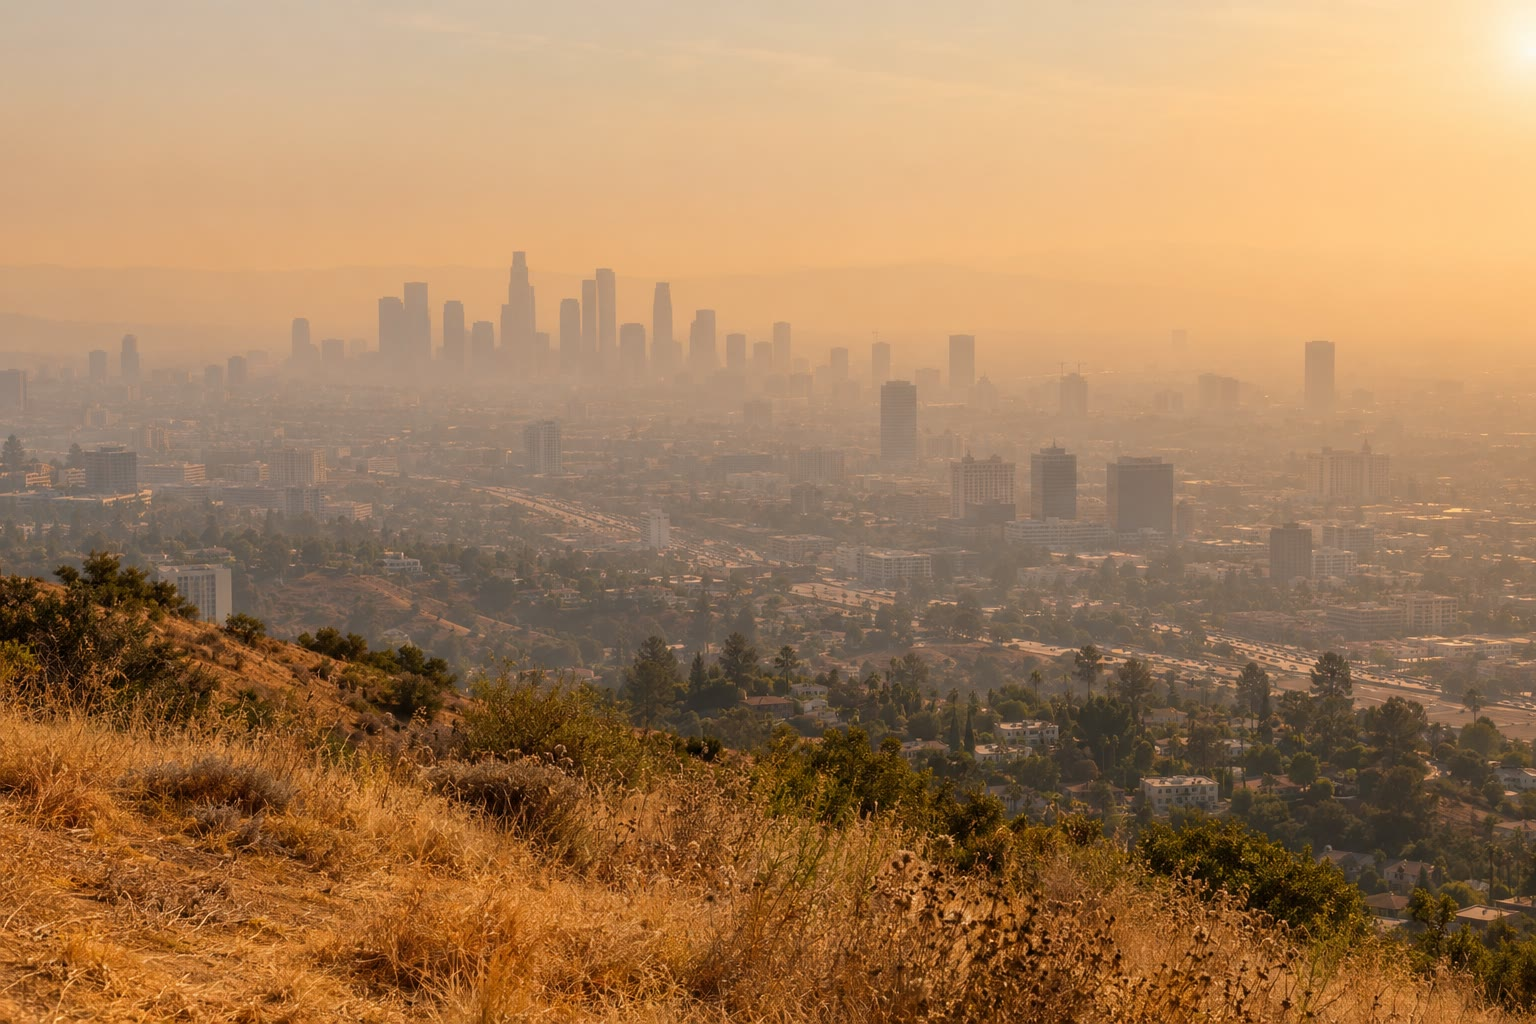
\includegraphics[width=0.6\linewidth]{images/book4/ai/b3-14-smog.jpg}

{\small 炎热午后，一座城市笼罩在\omterm{def:b3:photochemistry:smog}{光化学烟雾}中。褐色的色调
来自 \ce{NO2}；刺激肺部的臭氧则不可见。}
\end{omfigure}

\begin{omfigure}
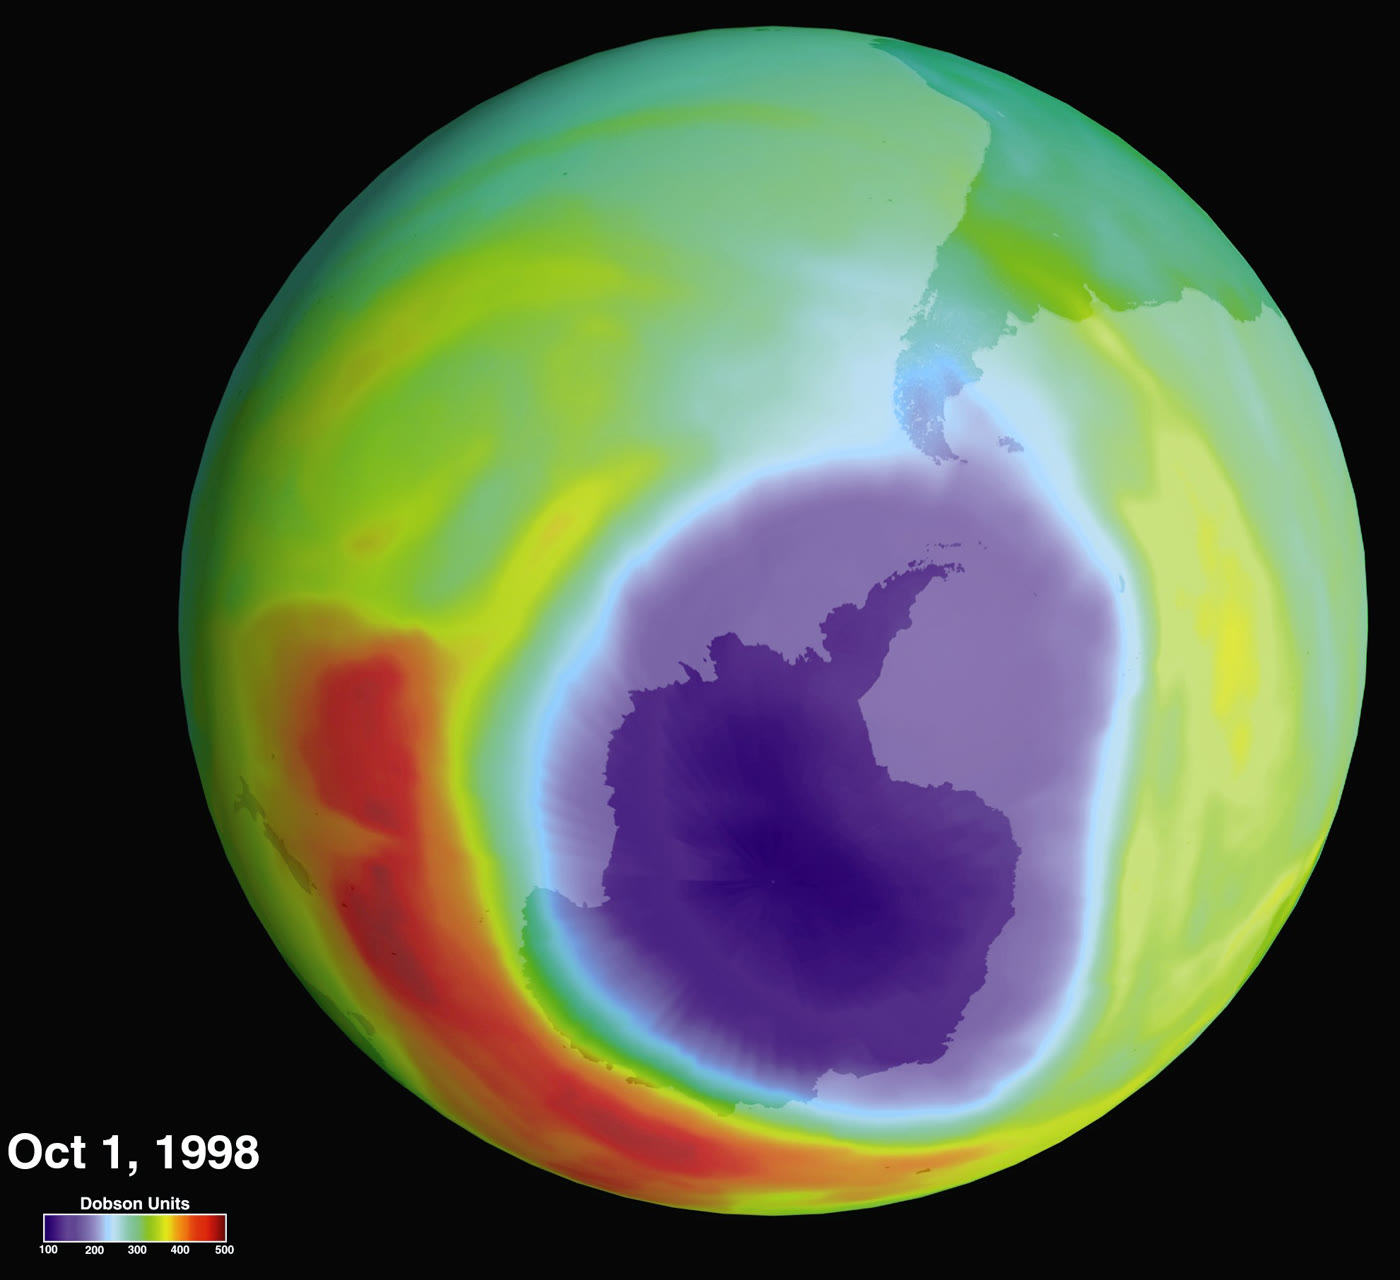
\includegraphics[width=0.5\linewidth]{images/book4/ozone-hole.jpg}

{\small 1998 年 10 月 1 日南半球上空的臭氧柱，由卫星测量得到：
南极上空的臭氧空洞（紫色）降至约
100 多布森单位，其他地区约为 300 多布森单位。}
\end{omfigure}

\begin{inthelab}[光反应器]
一盏中压汞灯，装于石英夹套中冷却，置于
反应容器的中心；一个玻璃滤光套管滤去
约 \qty{300}{nm} 以下的波长，以免破坏产物。溶液
经氮气流除氧（氧会淬灭\omterm{def:b3:many-electron-atoms:singlet-triplet}{三重态}）并搅拌。
整个反应器须加以封闭：灯发出的紫外线对眼睛
和皮肤有害，不得直视，即使只看一瞬间也不行。
\end{inthelab}

\begin{safety}{\ghs[0.8cm]{GHS08}\ghs[0.8cm]{GHS09}}
% ledger: ghs4:benzophenone
二苯甲酮是常用的\omterm{def:b3:photochemistry:sensitisation}{光敏剂}，也是光还原的反应物：
怀疑致癌，长期接触可能损害器官，
对水生生物有毒。称量和操作时须戴手套；残留物须放入
有机废物。
\end{safety}

\begin{history}[未来的光化学与天空中的空洞]
1912 年，贾科莫·恰米契安在博洛尼亚提出一个问题：工业是否有朝一日也能像植物那样，
靠阳光而非煤炭运转；他多年来一直在自己实验室的屋顶上，把装有有机化合物的烧瓶
放到太阳下曝晒。1985 年，
三位在南极一座科研站工作的科学家报告说，那里
春季的臭氧柱自 20 世纪 70 年代后期
起便急剧下降。
臭氧空洞在几年之内便由本章的化学原理得到解释，
进而促成了氟氯烃的逐步淘汰。
\end{history}

\section{练习}

\begin{exercise}[$\star$]\label{exo:b3:photochemistry:1}
一盏灯在 \qty{365}{nm} 处输出 \qty{100}{mW} 的功率。每秒有多少个光子，
以及每秒有多少爱因斯坦？
\end{exercise}

\begin{exercise}[$\star$]\label{exo:b3:photochemistry:2}
在 \qty{10.0}{min} 内，一份吸收速率为 \qty{1.00e-7}{einstein.s^{-1}} 的溶液
转化了 \qty{2.0e-5}{mol} 的反应物。求\omterm{def:b3:electronic-spectroscopy:quantum-yield}{量子产率}。
\end{exercise}

\begin{exercise}[$\star$]\label{exo:b3:photochemistry:3}
\ce{H2} 与 \ce{Cl2} 的光化学反应，其\omterm{def:b3:electronic-spectroscopy:quantum-yield}{量子产率}可高达 $10^4$ 乃至
更高。这说明了什么？请写出链增长步骤。
\end{exercise}

\begin{exercise}[$\star$]\label{exo:b3:photochemistry:4}
% ledger: janaf:O.dfH0, janaf:O3.dfH0
由 0 K 时 O（\qty{246.79}{kJ/mol}）和 \ce{O3}
（\qty{145.35}{kJ/mol}）的生成焓，求能使 \ce{O2} 分裂为两个
原子、以及使 \ce{O3} 分解为 \ce{O2} 和 O 的最长波长。
\end{exercise}

\begin{exercise}[$\star\star$]\label{exo:b3:photochemistry:5}
某光开关在 \qty{365}{nm} 处，$\varepsilon_E = 22\,000$ 及 $\varepsilon_Z = 1500$ \unit{L.mol^{-1}.cm^{-1}}，
且 $\Phi_{E\to Z} = 0.11$，$\Phi_{Z\to E} = 0.40$（习题数据）。求\omterm{def:b3:photochemistry:photoisomerisation}{光稳
态}组成。
\end{exercise}

\begin{exercise}[$\star\star$]\label{exo:b3:photochemistry:6}
写出己-2-酮的诺里什 II 型反应产物，并说明
为什么戊-2-酮生成乙烯而不是丙烯。
\end{exercise}

\begin{exercise}[$\star\star$]\label{exo:b3:photochemistry:7}
某受主的\omterm{def:b3:many-electron-atoms:singlet-triplet}{三重态}能量为 \qty{250}{kJ/mol}。在三种候选\omterm{def:b3:photochemistry:sensitisation}{光敏剂}中，
这三种候选\omterm{def:b3:photochemistry:sensitisation}{光敏剂}的\omterm{def:b3:many-electron-atoms:singlet-triplet}{三重态}能量分别为 289、253 和 \qty{236}{kJ/mol}（习题数据），
其中哪一种能高效地转移能量？估算
三者在 \qty{298}{K} 时各自的转移平衡常数。
\end{exercise}

\begin{exercise}[$\star\star$]\label{exo:b3:photochemistry:8}
% ledger: kin:O+O2+M.k0, kin:O+O2+M.n
在 \qty{230}{K} 下，$[\mathrm M] = \qty{4.0e17}{cm^{-3}}$，$[\ce{O2}] = 0.21[\mathrm M]$，且 $j_3 = \qty{1.0e-3}{s^{-1}}$，
求 $k_2$ 及稳态时的比值 $[\ce{O}]/[\ce{O3}]$。
\end{exercise}

\begin{exercise}[$\star\star$]\label{exo:b3:photochemistry:9}
% ledger: kin:Cl+O3.A, kin:Cl+O3.EaR, kin:Cl+CH4.A, kin:Cl+CH4.EaR
在 \qty{230}{K} 下，求 $\ce{Cl + O3}$ 与 $\ce{Cl + CH4}$ 的速率常数，以及
一个 Cl 原子遇到 \ce{O3} 而非 \ce{CH4} 的概率（设 $[\ce{O3}] = \qty{5.7e12}{cm^{-3}}$，
$[\ce{CH4}] = \qty{4.0e11}{cm^{-3}}$）。
\end{exercise}

\begin{exercise}[$\star\star\star$]\label{exo:b3:photochemistry:10}
% ledger: kin:NO+O3.A, kin:NO+O3.EaR
某城市正午时，$[\ce{NO2}]/[\ce{NO}] = 1.5$，$j_{\ce{NO2}} = \qty{8.0e-3}{s^{-1}}$。
求 \qty{298}{K} 时的\omterm{def:b3:photochemistry:photoisomerisation}{光稳态}臭氧浓度，分别以分子每 \unit{cm^3} 和 ppb 表示（空气处于 \qty{1}{bar}）。
夜晚会发生什么？
\end{exercise}

\begin{exercise}[$\star\star\star$]\label{exo:b3:photochemistry:11}
一份 \qty{3.0}{mL}、在 \qty{313}{nm} 处吸光度为 0.50 的溶液，
受到该波长的 \qty{50}{mW} 光照射；反应的 $\Phi = 0.25$。求以
\unit{mol.L^{-1}.s^{-1}} 表示的初始速率。
\end{exercise}

\begin{exercise}[$\star\star\star$]\label{exo:b3:photochemistry:12}
一个草酸铁\omterm{def:b3:photochemistry:photon-flux}{化学光量计}，在 \qty{365}{nm} 处\omterm{def:b3:electronic-spectroscopy:quantum-yield}{量子产率}为 1.25（习题
数据），全部吸收入射光，在 \qty{60}{s} 内生成 \qty{3.0e-6}{mol} 的 Fe(II)。
求\omterm{def:b3:photochemistry:photon-flux}{光子通量}。为什么转化率必须保持较小？
\end{exercise}

\section{问题：臭氧层的形成与耗损}

\begin{problem}[{周末问题——臭氧层的形成与耗损：光子阈值，
采用计算所得速率常数的查普曼机理稳态、
氯循环，以及使其停止的储库物种}]
\label{pb:b3:photochemistry:1}
% ledger: janaf:O.dfH0, janaf:O3.dfH0, kin:O+O2+M.k0, kin:O+O2+M.n, kin:O+O3.A, kin:O+O3.EaR, kin:Cl+O3.A, kin:Cl+O3.EaR, kin:O+ClO.A, kin:O+ClO.EaR, kin:Cl+CH4.A, kin:Cl+CH4.EaR, kin:ClO+NO2+M.k0, kin:ClO+NO2+M.n, kin:ClO+NO2+M.kinf, kin:ClO+NO2+M.Fc, oz:column.mean, oz:column.hole
一个平流层模型，高度约 \qty{30}{km}（本题数据）：$T = \qty{230}{K}$，$[\mathrm M] =
\qty{4.0e17}{cm^{-3}}$，$[\ce{O2}] = 0.21[\mathrm M]$，\omterm{def:b3:photochemistry:photolysis}{光解速率常数} $j_1 = \qty{1.0e-11}{s^{-1}}$（\ce{O2}）
及 $j_3 = \qty{1.0e-3}{s^{-1}}$（\ce{O3}），$[\ce{CH4}] = \qty{4.0e11}{cm^{-3}}$，$[\ce{NO2}] = \qty{1.0e9}{cm^{-3}}$。计算所得速率常数
（单位为 \unit{cm^3.s^{-1}}，$k_2$ 为 \unit{cm^6.s^{-1}}，浓度按每 \unit{cm^3} 计）：
$k_2 = \num{6.0e-34}(T/300)^{-2.6}$; $k_4 = \num{8.0e-12}\eu^{-2060/T}$; Cl + \ce{O3}: $\num{2.8e-11}\eu^{-250/T}$;
O + ClO：$\num{2.5e-11}\eu^{110/T}$；Cl + \ce{CH4}：$\num{6.6e-12}\eu^{-1240/T}$；ClO + \ce{NO2} + M：$\num{1.41e-13}$，在
此条件下。

\medskip\noindent\textbf{第一部分——光子阈值。}
\begin{enumerate}
  \item 求 $D_0(\ce{O2})$，已知 $\Delta_fH^\circ_0(\ce{O}) = \qty{246.79}{kJ/mol}$。
  \item 由此求能使 \ce{O2} 分裂的最长波长。
  \item 求 $\ce{O3 -> O2 + O}$ 的能量（$\Delta_fH^\circ_0(\ce{O3}) = \qty{145.35}{kJ/mol}$），及其
        阈值波长。
  \item 可见光原则上也能分解臭氧；那么为什么对生命至关重要的，是臭氧的
        紫外吸收？
  \item 为什么 \ce{O2} 只在大气高层发生\omterm{def:b3:photochemistry:photolysis}{光解}？
\end{enumerate}

\medskip\noindent\textbf{第二部分——查普曼稳态。}
\begin{enumerate}[resume]
  \item 写出查普曼的四个步骤。
  \item 求 $k_2$ 和 $k_2[\mathrm M]$，温度为 \qty{230}{K}。
  \item 求 $k_4$。
  \item 求 $[\ce{O}]/[\ce{O3}]$。
  \item 证明 $[\ce{O3}] = [\ce{O2}]\sqrt{j_1k_2[\mathrm M]/(j_3k_4)}$。
  \item 求 $[\ce{O3}]$ 及其混合比。
  \item 求 $[\ce{O}]$。
  \item 观测到的臭氧量低于此值，原因何在？
\end{enumerate}

\medskip\noindent\textbf{第三部分——氯循环。}
\begin{enumerate}[resume]
  \item 写出该循环及其总反应。
  \item 求氯原子相对于 \ce{O3} 的寿命。
  \item 求 ClO 相对于 O 的寿命。
  \item 由此推出稳态比值 $[\ce{ClO}]/[\ce{Cl}]$。
  \item 已知 $[\ce{Cl}] + [\ce{ClO}] = \qty{1.0e7}{cm^{-3}}$，比较该循环
        造成的奇氧损失速率与查普曼步骤 $\ce{O + O3}$ 的速率。
  \item 哪一步限制了整个循环？
\end{enumerate}

\medskip\noindent\textbf{第四部分——\omterm{def:b3:photochemistry:ozone-depletion}{储库物种}。}
\begin{enumerate}[resume]
  \item 求氯原子与 \ce{O3} 反应而不与
        \ce{CH4} 反应的概率。
  \item 求 ClO 与 O 反应而非与 \ce{NO2} 反应的概率。
  \item 由此推出循环完成一轮的概率 $p$。
  \item 由此推出氯被捕获前循环的平均轮数。
  \item 解释极地平流层云如何延长反应链。
  \item 给出结论：一个氯原子在本模型中
        被\omterm{def:b3:photochemistry:ozone-depletion}{储库物种}捕获之前能破坏的臭氧分子数。
\end{enumerate}
\end{problem}
